\documentclass[intlimits,twoside,a4paper,11pt]{article}

\usepackage[utf8]{inputenc}
\usepackage[T2A]{fontenc}
%Здесь порядок языков наоборот! Сначала русский, потом английский
\usepackage[russian,english]{babel}

%Здесь дописана дополнительная опция english
\usepackage[eqsecnum,english]{kioj}

\setcounter{page}{42}

\journalsectionnoimage{}
\issue{2015}{-}{edu}
\udknumber{621.320}

\title[Paper title]{PAPER TITLE}

\authorI[Andreev А.]{Andreev Andrew}
\authorIaddr{Ph.D. at MIT}
\authorIemail{aaa@org.com}

\authorII[Borisov B.]{Borisov Boris}
\authorIIaddr{Ph.D. at MIT}
\authorIIemail{bbb@org.com}

\begin{document}

\maketitle

\begin{abstract}
An abstract in English. Some abstract in English. An abstract in English. Some abstract in English. An abstract in English. Some abstract in English. An abstract in English. Some abstract in English. An abstract in English. Some abstract in English. An abstract in English. Some abstract in English. An abstract in English. Some abstract in English. An abstract in English. Some abstract in English. An abstract in English. Some abstract in English.
\keywords keywords in English, more keywords in English
\end{abstract}

\section{INTRODUCTION}
Some English text, some English text, Some English text, some English text, Some English text, some English text, Some English text, some English text, Some English text, some English text, with proper hyphenation. Very extermination extermination extermination extermination extermination extermination extermination extermination word, and anyway with the hyphenation.

\section{FIRST SECTION}
Some English text, some English text, Some English text, some English text, Some English text, some English text, Some English text, some English text, Some English text, some English text, with proper hyphenation.
\begin{itemize}
\item Itemization exmaple.
\item The second point.
\item The third point.
\end{itemize}

And now for something completely different:
\begin{enumerate}
\item The first point;
\item The second point;
\item The third point.
\end{enumerate}
Reference to the image~\ref{fig-example}

\begin{figure}[htb]
\centering
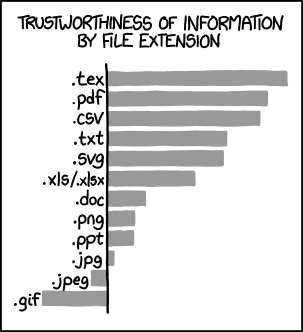
\includegraphics[width=0.4\textwidth]{xkcd1301.png}
\caption{Достоверность информации в зависимости от расширения файла} \label{fig-example}
\end{figure}

\begin{table}[H]
\centering
\caption{Table example}
\label{table-example}
\begin{tabular}{|c|c|}
	\hline
	Question & ? \\
	\hline
	Answer & 42 \\
	\hline
\end{tabular}
\end{table}

\subsection{Подраздел}
Text in subsection
\subsubsection{Подподраздел}
Text in subsection with an example of an image consisting of two images. We can reference the full image, for example,~\ref{fig-example-2}, or subimages, for example,~\ref{fig-example-2b}.

\begin{figure}[H]
	\centering
	\begin{subfigure}[t]{70mm} %указываем размер подрисунка, без буквы [t] картинки будут вертикально отцентрованы
		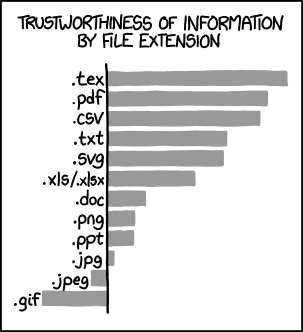
\includegraphics[width=\textwidth]{xkcd1301.png} %width=\textwidth указывает, что ширина совпадает с шириной подрисунка
		\subcaption{Необязательный подзаголовок}
		\label{fig-example-2a}
	\end{subfigure}
	\quad %это широкий пробел между двумя рисунками
	\begin{subfigure}[t]{50mm}
		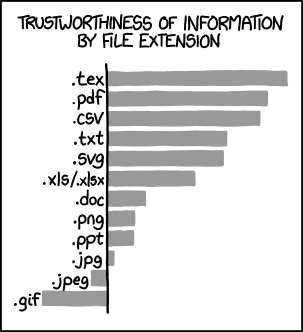
\includegraphics[width=\textwidth]{xkcd1301.png}
		\subcaption{} % Здесь подзаголовок не указан
		\label{fig-example-2b}
	\end{subfigure}
	\caption{Пример двух изображений рядом на одном рисунке} \label{fig-example-2}
\end{figure}

\section{CONCLUSION}
Some conslusion text with a reference:~\cite{lib-1,lib-2}

\begin{thebibliography}{9}
\bibitem{lib-1} {\it Madhav S.} Game Programming Algorithms and Techniques: A Platform-Agnostic Approach (Game Design). UK, 2013. 
\bibitem{lib-2} {\it Ericson C.} Real-Time Collision Detection. USA, 2004.
\end{thebibliography}

\translatedpart

\title{Русский заголовок}
\author{Андреев А., Борисов Б.}

\maketranslatedtitle

\begin{abstract}
Русский текст аннотации, русский текст аннотации, русский текст аннотации, русский текст аннотации, русский текст аннотации, русский текст аннотации.
\keywords руские ключевые слова, разделенные запятыми
\end{abstract}

\makekioauthors

\end{document}
